\section{Présentation des objectifs du stage}
        \subsection{Contexte}
            \paragraph*{}
            De nos jours, dans le contexte de l'industrialisation et de la numérisation des productions, il est important d'avoir des réponses automatisées afin de gagner en flexibilité et en compétitivité. Une automatisation de ce type repose donc sur des systèmes et des équipements très hétérogènes que ce soit dans les systèmes employés, les informations à analyser ou encore les protocoles réseaux utilisés.
            
            Ces infrastructures reposent sur des systèmes cyber-physiques. Bien que ces infrastructures assurent une traçabilité très précise de la chaîne de production, les informations récoltées peuvent ne pas suffire afin d'identifier un potentiel problème et son origine.
            
            \paragraph*{}
            Les domaines d'applications des drones peuvent être très divers et peuvent être complémentaires à d'autres systèmes de reconnaissance déjà présent. Les drones peuvent par exemple être utilisés dans la surveillance de l'infrastructure ou encore compléter des diagnostics qui peuvent être réalisés à distance par des opérateurs en cas de panne. Les drones étant équipés de caméra et pouvant se déplacer librement sans interférer avec le processus de fabrication, ils sont des atouts indispensables pour prendre des images de la panne et les envoyer aux opérateurs pour le traitement, l'analyse et le recouvrement de la panne.
            
            \paragraph*{}
            Lorsque le drone se déplace pour aller jusqu'à la panne, il doit être en mesure de se localiser précisément afin de s'y rendre le plus rapidement possible tout en évitant de causer des dommages corporels avec du personnel se trouvant sur le chemin. Pour se faire, le drone doit être synchronisé avec la chaîne de production et utiliser des algorithmes de détection de panne qui seraient implantés directement dans le système afin de l'avertir d'une panne immédiate ou d'une potentielle menace de panne si des algorithmes de maintenances sont utilisés.
            
		\subsection{Problématique}
		    \paragraph*{}
		    La problématique de ce stage est d'assurer une coopération entre les dispositifs présents tels que la chaine de production, les automates et le drone ainsi que d'assurer différentes opérations comme la prise d'image d'une panne au sein de la plateforme ou encore la surveillance de l'environnement afin d'éviter des risques pour le personnel ou les équipements.
		
        \subsection{Fonction principale}
            \paragraph*{}
            Ce stage s'est composé de trois grandes étapes principales.
            
            \paragraph*{}
            La première étape était la découverte de l'environnement. Cette étape a consisté à comprendre le fonctionnement des automates et de la plateforme. La compréhension de l'environnement s'est faite grâce aux protocoles réseaux, au système, et les langages de programmation utilisés. J'ai ainsi découvert le fonctionnement d'un automate programmable ainsi que le protocole de communication ModBus TCP/IP.
            
            \paragraph*{}
            La seconde étape a été la connexion du drone à la partie industrielle (la plateforme). Le laboratoire Lab-STICC possède un drone de la marque DJI : le drone Matrice 100 (M100)\cite{djiMat100}. Il m'a fallu analyser les capteurs du drone ainsi que trouver une solution afin de le piloter dans l'espace contraint de la pièce représentant l'industrie. Le drone pouvait être équipé de cartes de communication sans fil afin d'intéragir avec la plateforme, d'une caméra afin de prendre des photos des dispositifs, ou de tout autre équipement nécessaire au bon fonctionnement du drone dans la pièce par rapport à nos besoins.
            
            \paragraph*{}
            La dernière étape était l'analyse de données par le drone. Le but était ainsi de créer une interaction entre le drone et la plateforme afin que le drone se déplace d'un point initial vers un point où se trouve une panne qui a été détectée ou estimée, puis prendre des photos de la panne et les envoyer aux opérateurs. Le chemin que prend le drone doit être calculé afin qu'il ne comporte aucun risque pour l'environnement (personnels ou équipements).
            
            
            \begin{figure}[H]
                \centering
                \begin{frame}{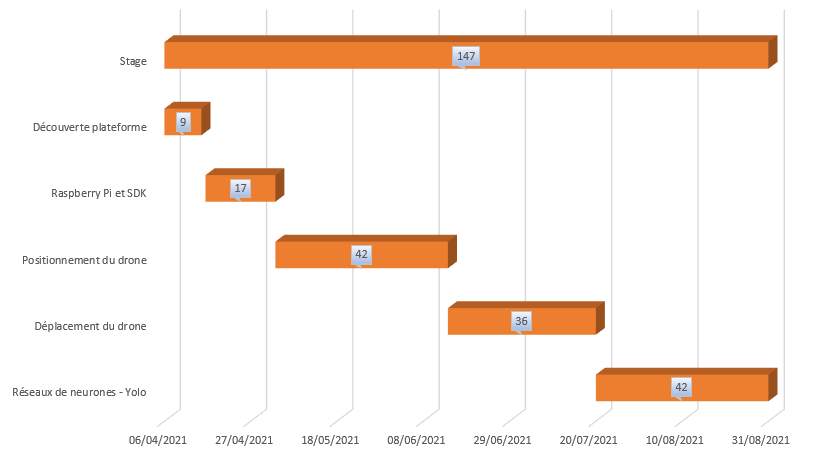
\includegraphics[width=1\textwidth]{image/gantt.png}}
                \end{frame}
                \caption{\label{fig:gantt}Diagramme de Gantt représentant le temps passé sur chacune des étapes}
            \end{figure}
            
        \subsection{L'existant}
            \subsubsection{La plateforme}
            \label{part-automate}
                \begin{figure}[H]
                    \centering
                    \begin{frame}{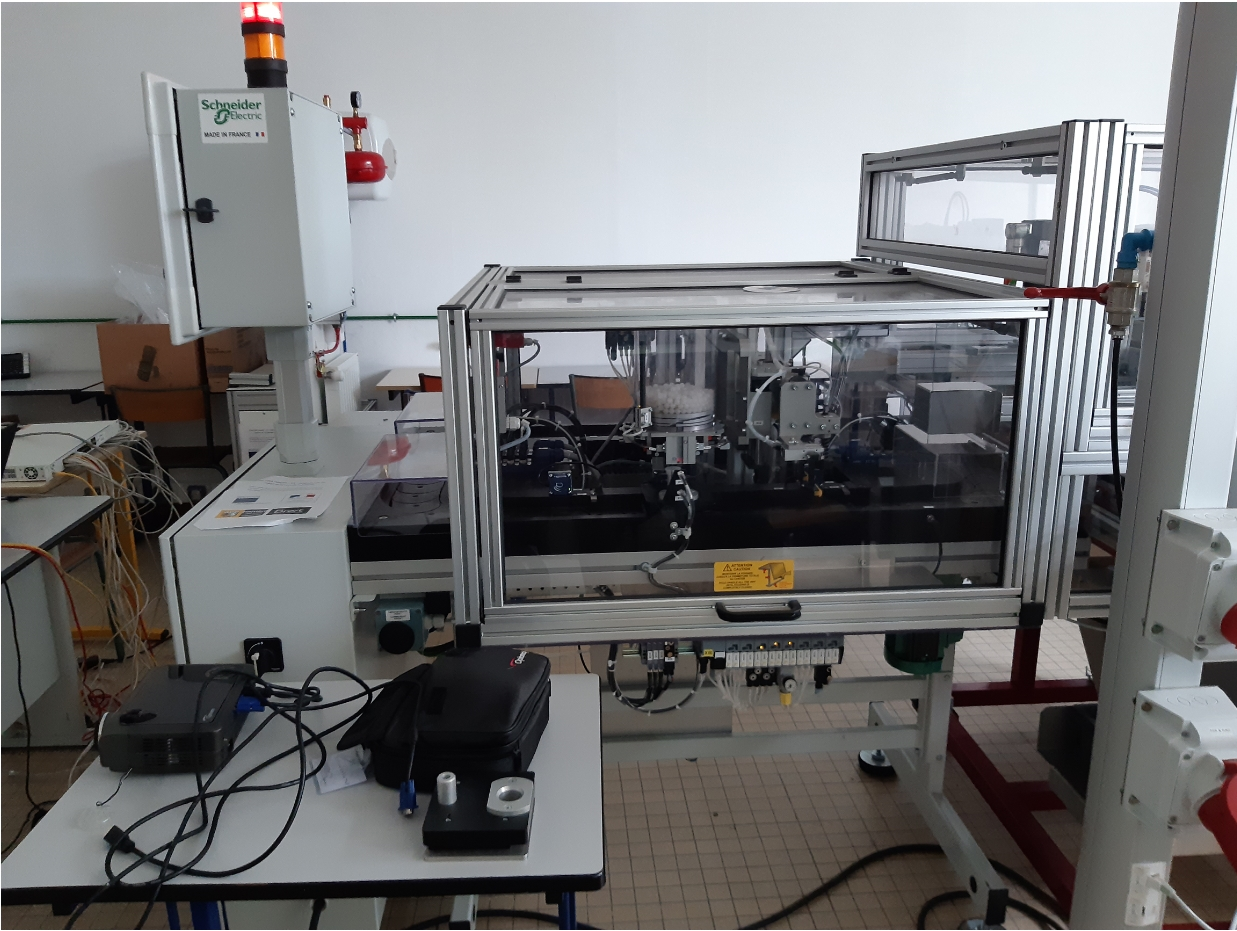
\includegraphics[width=1\textwidth]{image/plateforme.jpg}}
                    \end{frame}
                    \caption{\label{fig:plateforme}Plateforme industrielle}
                \end{figure}
                
                \paragraph*{}
                Nous avons à disposition au laboratoire une réplique de plateforme (voir figure \ref{fig:plateforme}) d'un complexe d'industrie pharmaceutique. Cette plateforme est conçue initialement par Schneider Electric. Elle se décompose en deux modules comportant chacun un automate de la même marque (automate M340 et M580). Un exemple de l'intérieur de l'automate se trouve sur la figure \ref{fig:int-automate}.
                
                \begin{figure}[H]
                    \centering
                    \begin{frame}{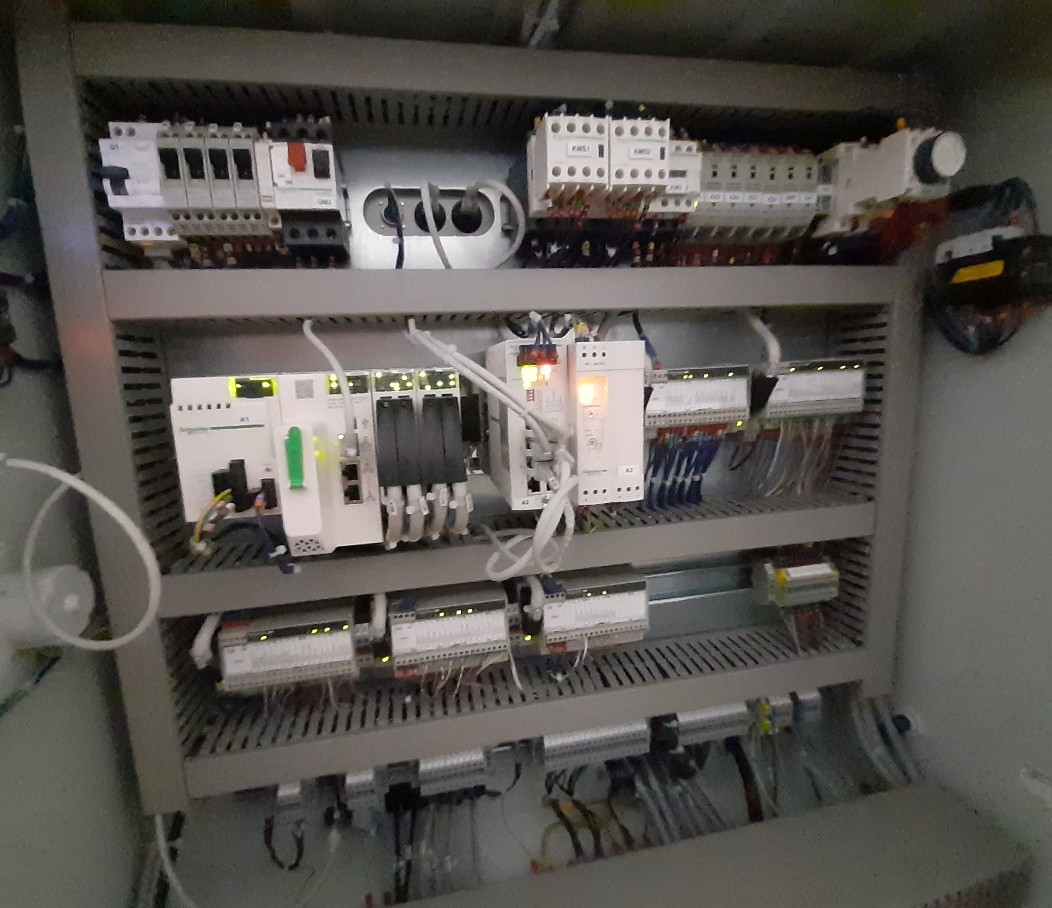
\includegraphics[width=1\textwidth]{image/automate.jpg}}
                    \end{frame}
                    \caption{\label{fig:int-automate}Intérieur d'un automate}
                \end{figure}
                
                \paragraph*{}
                Le premier module s'occupe de la gestion des commandes (recettes) dictées par l'utilisateur. Une fois une commande réalisée, un bras articulé va venir récupérer un flacon et un bouchon puis va les déposer sur une palette. Ensuite, cette palette va passer sur un convoyeur et aller dans le deuxième module. Lorsque la palette revient du second module, le bras articulé récupère le flacon bouché et met ce flacon dans un carton. Une fois que le carton est plein, un convoyeur amène le carton dans un autre endroit afin d'y être stocké.
                
                \paragraph*{}
                Le second module s'occupe du traitement de la commande. La commande est traitée par des puces RFID qui se trouvent tout au long de la chaîne de production. La commande consiste à mettre des billes dans le flacon. La quantité de billes à mettre dépend de la commande. Comme on peut voir sur la figure \ref{fig:module-plateforme}, la partie gauche avec le réservoir de bille et à droite l'appareil qui va refermer le flacon avec le bouchon mis sur la palette.
                
                \begin{figure}[H]
                    \centering
                    \begin{frame}{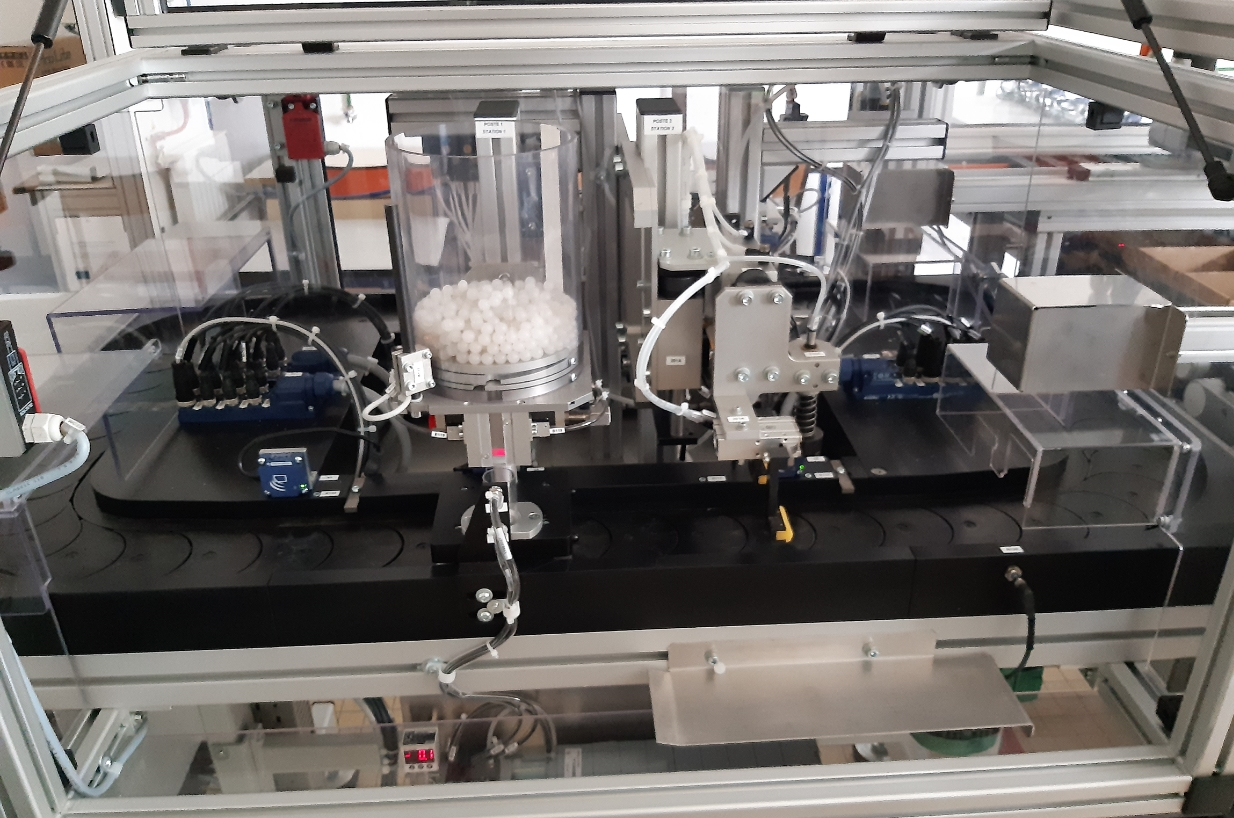
\includegraphics[width=1\textwidth]{image/vueensemble.jpg}}
                    \end{frame}
                    \caption{\label{fig:module-plateforme}Module secondaire de la plateforme}
                \end{figure}

            \subsubsection{Le drone}
            \label{part:existDrone}
				\paragraph*{}
				Le drone possédé par le laboratoire est le matrice M100 de la marque DJI. Ce drone est optimal pour le monde de la recherche car il possède de nombreux capteurs, un bon autopilote, de nombreux tutoriels et également la possibilité d'embarquer davantage de matériels comme une caméra, des batteries, un ordinateur embarqué, etc. L'entreprise DJI met à disposition des outils afin d'accéder aux capteurs, autopilote et autres fonctionnalités de leurs drones. Ces outils peuvent être appliqués pour créer une application Android/iOS pour manipuler le drone, gérer les capteurs/appareils ajoutés au drone, ou encore de connecter son propre ordinateur embarqué à un drone compatible par le port série ($UART$).
				
				Selon le besoin de ce stage, j'ai utilisé l'outil fourni par DJI s'appellant Onboard-SDK\cite{githubSDK}. Cet outil permet de connecter un ordinateur embarqué sur le drone et d'accéder aux capteurs, à l'autopilote et de manipuler le drone à distance de manière automatique et programmable directement dans l'ordinateur en C++. Il existe de nombreux exemples sur le site du constructeur afin de faire fonctionner ce $SDK$ sur le drone de notre choix. Le choix de la version du $SDK$ est déterminé par le drone. Nous utilisons un drone Matrice 100 dont la dernière version du $SDK$ compatible est la version 3.9 du $SDK$. Les versions suivantes peuvent être compatibles également mais elles ne sont pas indiqué comme tel sur le site du constructeur et donc afin d'anticiper un quelconque problème de compatibilité j'ai préféré prendre la version recommandée par le constructeur.
				
				\begin{figure}[H]
        		    \centering
        		    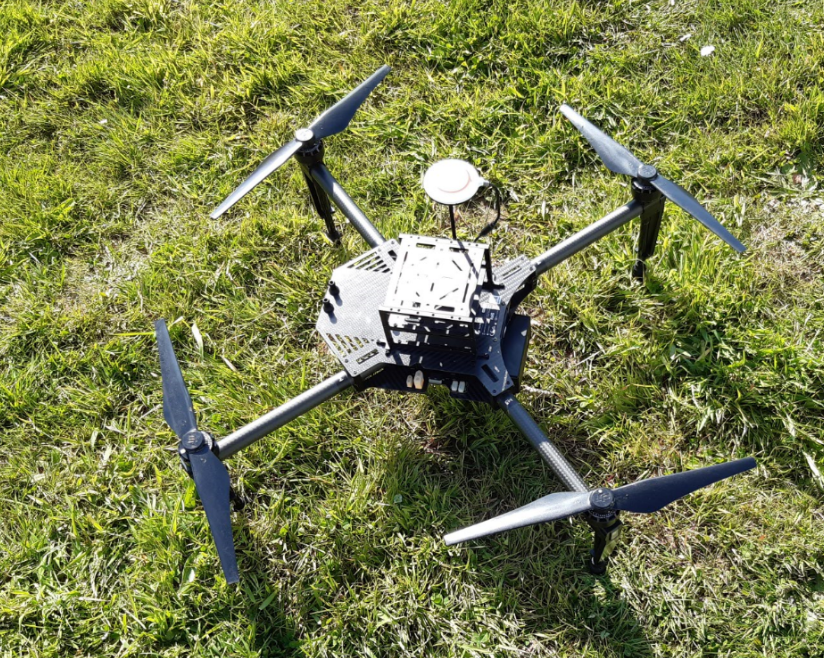
\includegraphics[width=1\textwidth]{image/drone.png}
        		    \caption{Matrice 100 vue aérienne}
        		    \label{fig:drone}
		        \end{figure}